\documentclass[12pt]{article}
\usepackage{amsmath}
\usepackage{amsfonts}
\usepackage{graphicx}
\usepackage{float}
\begin{document}
\title{Electrical Engineering 113, Homework 1}
\date{April 8th, 2019}
\author{Michael Wu\\UID: 404751542}
\maketitle

\section*{Problem 1}

\paragraph{a)}

\[g_1[n]=(n-3)(u[n+1]-u[n-8])\]
\begin{figure}[H]
    \begin{center}
        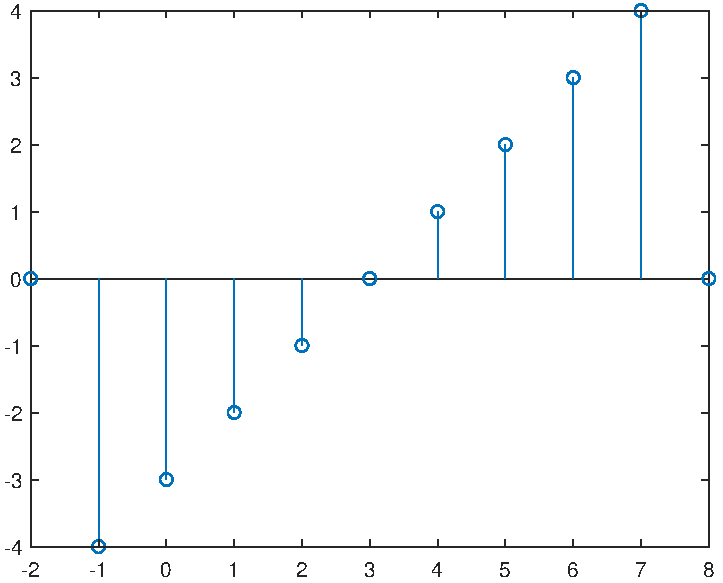
\includegraphics[width=3.3in]{problem1a.pdf}
    \end{center}
\end{figure}

\pagebreak

\paragraph{b)}

\[g_2[n]=(2n-3)(u[2n+1]-u[2n-8])\]
\begin{figure}[H]
    \begin{center}
        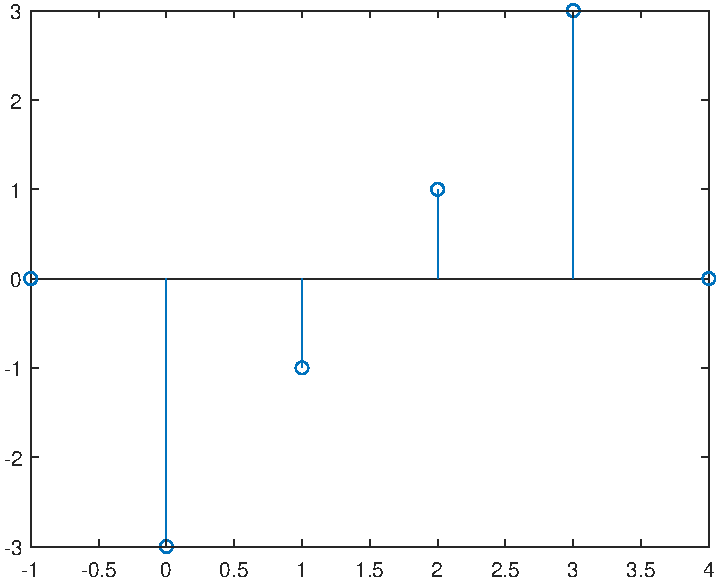
\includegraphics[width=3.3in]{problem1b.pdf}
    \end{center}
\end{figure}

\paragraph{c)}

\[g_3[n]=-n(u[-n+4]-u[-n-5])\]
\begin{figure}[H]
    \begin{center}
        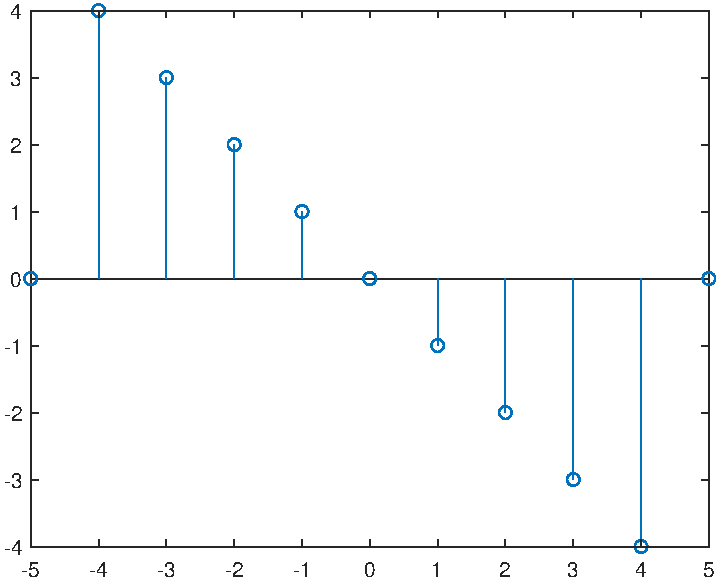
\includegraphics[width=3.3in]{problem1c.pdf}
    \end{center}
\end{figure}

\paragraph{d)}

\[g_4[n]=(2-n)(u[-n+6]-u[-n-3])\]
\begin{figure}[H]
    \begin{center}
        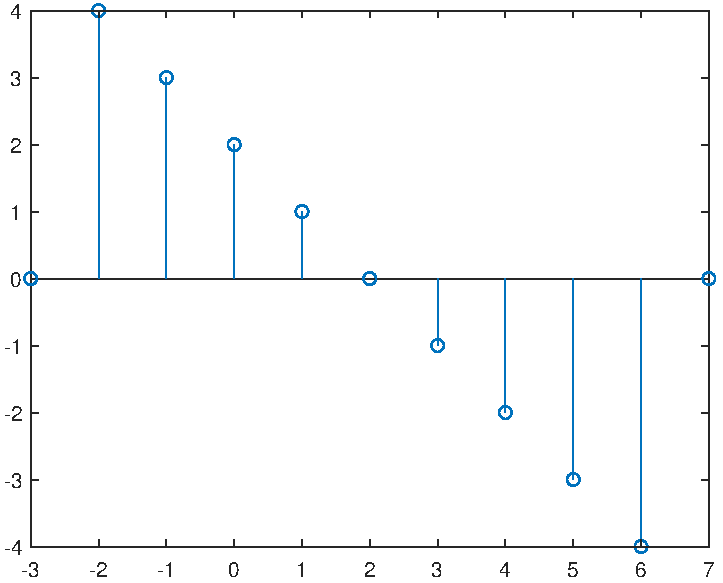
\includegraphics[width=3.3in]{problem1d.pdf}
    \end{center}
\end{figure}

\paragraph{e)}

\[g_5[n]=\begin{cases}
    \frac{n}{2}\left(u\left[\frac{n}{2}+4\right]-u\left[\frac{n}{2}-5\right]\right) & \frac{n}{2}\in\mathbb{Z}\\
    0 & \text{otherwise}
\end{cases}\]
\begin{figure}[H]
    \begin{center}
        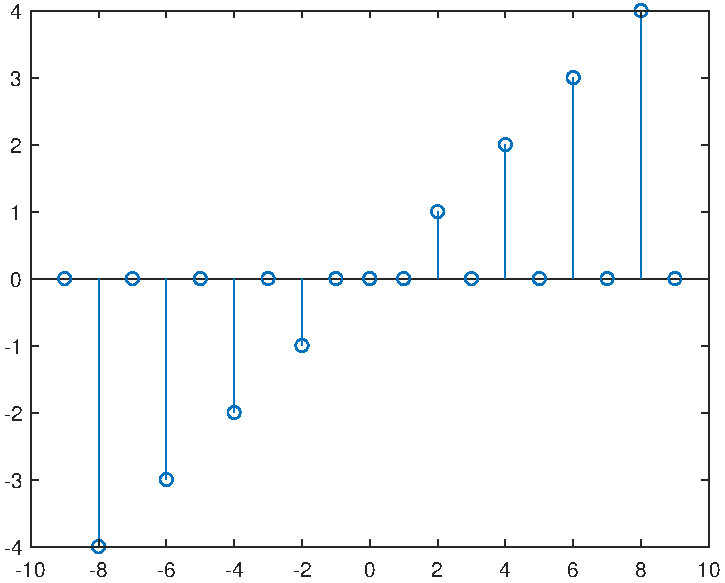
\includegraphics[width=3.3in]{problem1e.pdf}
    \end{center}
\end{figure}

\paragraph{f)}

\[g_6[n]=0\]
\begin{figure}[H]
    \begin{center}
        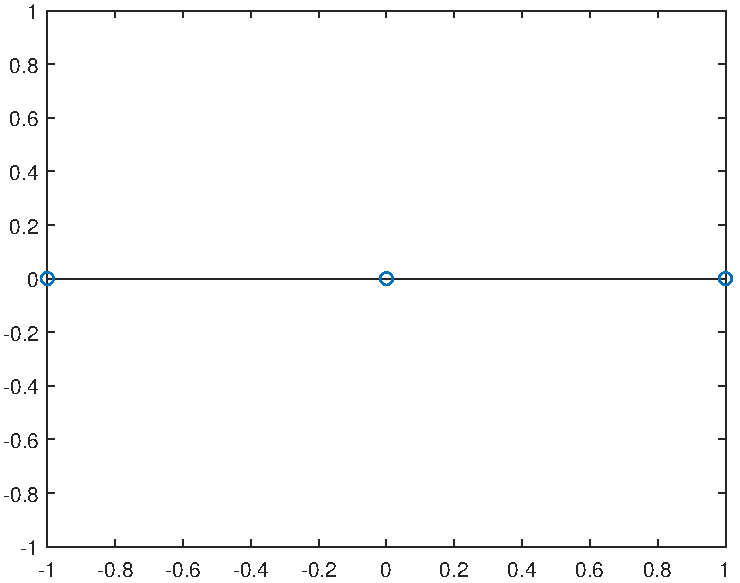
\includegraphics[width=3.3in]{problem1f.pdf}
    \end{center}
\end{figure}

\section*{Problem 2}

\paragraph{a)}

The plot of \(x[n]\) is shown below.
\begin{figure}[H]
    \begin{center}
        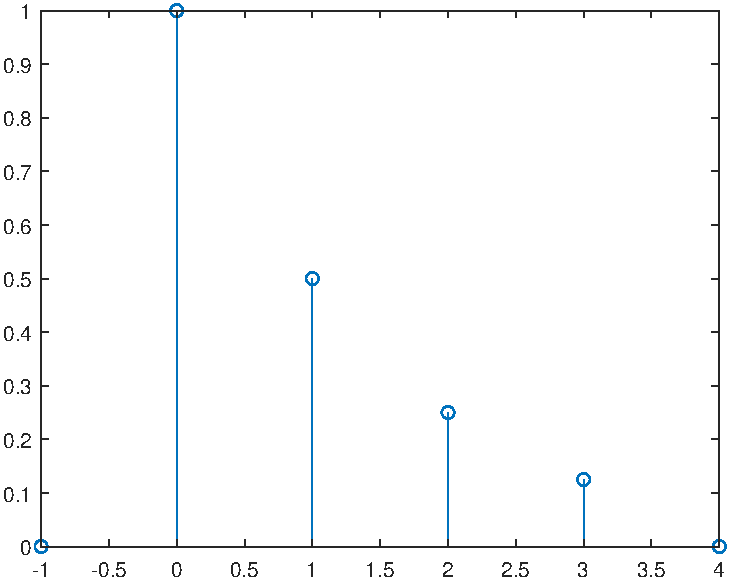
\includegraphics[width=3.3in]{problem2ax.pdf}
    \end{center}
\end{figure}
The plot of \(y[n]\) is shown below.
\begin{figure}[H]
    \begin{center}
        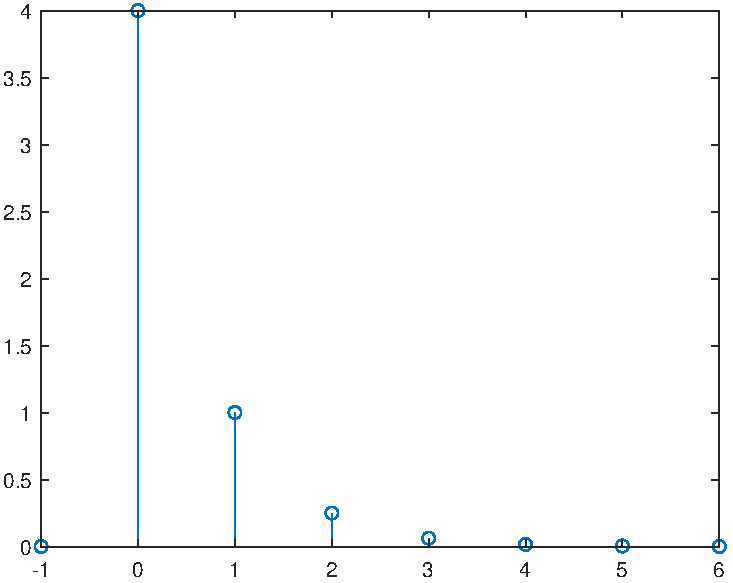
\includegraphics[width=3.3in]{problem2ay.pdf}
    \end{center}
\end{figure}

\paragraph{b)}

The plot of \(z[n]\) is shown below
\begin{figure}[H]
    \begin{center}
        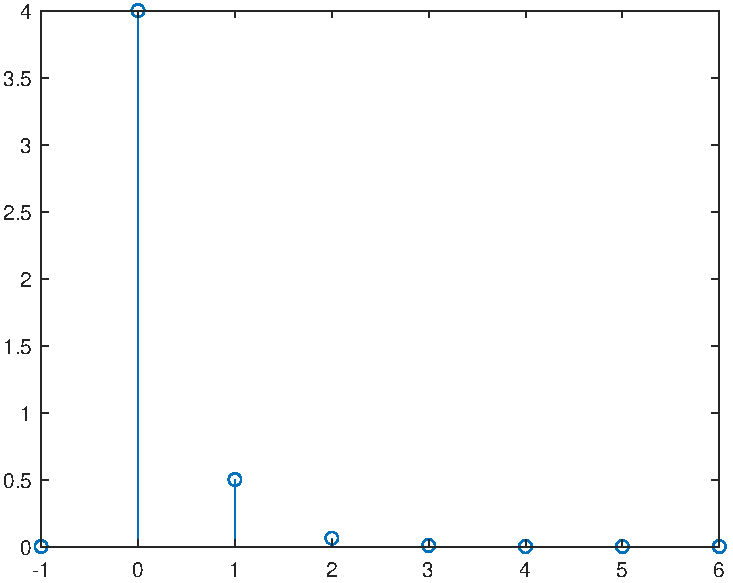
\includegraphics[width=3.3in]{problem2b.pdf}
    \end{center}
\end{figure}

\paragraph{c)}

The energy of \(x[n]\) is equal to the following value.
\[1^2 + \left(\frac{1}{2}\right)^2 + \left(\frac{1}{2}\right)^4 + \left(\frac{1}{2}\right)^6 = \frac{85}{64} = 1.328125\]
The energy of \(z[n]\) is equal to the following value.
\[4^2 + \left(\frac{1}{2}\right)^2 + \left(\frac{1}{2}\right)^8 + \left(\frac{1}{2}\right)^{14} = \frac{266305}{16384} \approx 16.254\]

\section*{Problem 3}

\paragraph{a)}

This is not periodic since the normalized frequency does not contain \(\pi\) and so the value of \(x[n]\) will be different for all \(n\).

\paragraph{b)}

The left sinusoid has a fundamental period of \(25\) and the right sinusoid has a fundamental period of \(5\). Thus the overall fundamental
period is \(25\).

\section*{Problem 4}

We have that \(x[n] = x_e[n] + x_o[n]\). By linearity the DC component of \(x[n]\) is the sum of the DC component of its even and odd components.
The odd component is \(0\) at \(n=0\), so we can rewrite the DC level as the following.
\[\lim_{N\to\infty} \left(\frac{1}{2N+1}\sum_{n=1}^N x[n] + x[-n]\right)\]
Since the definition of an odd function has that \(x[n] = -x[-n]\), this expression becomes zero. Thus the DC component of \(x[n]\) is equal
to only the DC component of \(x_e[n]\).

\section*{Problem 5}

\paragraph{a)}

We have that \(x_1[n] = x_1[-n]\) and \(x_2[n] = x_2[-n]\). Then we have the following.
\[x[n]=x_1[n]x_2[n]=x_1[-n]x_2[-n]=x[-n]\]
Therefore \(x[n]\) is even.

\paragraph{b)}

We have that \(x_1[n] = -x_1[-n]\) and \(x_2[n] = -x_2[-n]\). Then we have the following.
\[x[n]=x_1[n]x_2[n]=x_1[-n]x_2[-n]=x[-n]\]
Therefore \(x[n]\) is even.

\paragraph{c)}

We have that \(x_1[n] = x_1[-n]\) and \(x_2[n] = -x_2[-n]\). Then we have the following.
\[x[n]=x_1[n]x_2[n]=-x_1[-n]x_2[-n]=-x[-n]\]
Therefore \(x[n]\) is odd.

\section*{Problem 6}

Since our initial conditions at \(n=0\) match, we can solve the recursion for \(n>0\).
\begin{align*}
    \bar{x}[n-1] &= \frac{1}{n}\sum_{k=0}^{n-1}x[k]\\
    \bar{x}[n] &= \frac{n}{n+1}\frac{1}{n}\sum_{k=0}^{n-1}x[k] + \frac{1}{n+1}x[n]\\
    \bar{x}[n] &= \frac{1}{n+1}\left(\sum_{k=0}^{n-1}x[k] + x[n]\right)\\
    \bar{x}[n] &= \frac{1}{n+1}\sum_{k=0}^n x[k]
\end{align*}
This matches our given definition of \(\bar{x}[n]\), so it is a valid solution for the recursion.

\end{document}